\section{Methodology}

We expect some level of standardization (i.e. method names or status codes) or some commonalities such as user names, device details, semantic contexts, and other conversation or implementation-specific indicators even in highly entropic or variable packet data. Using this hypothesis, \textsc{Maple} transforms packets into grayscale images which will appear similar to one another. Thus, machine learning algorithms designed for image analysis may record the hidden features generated from the similarities between the two images. We base this assumption on previous work~\cite{lim2019network} which has shown similarities in grayscale images rendered from packet data in order to classify traffic by application and protocol type which are detectable by CNNs. Figure~\ref{fig:grayscale} asserts the validity of this assumption by showing comparative images rendered from packets in our combined dataset previously used and explained in detail in chapter 4 of this work.

\begin{figure} [ht!]
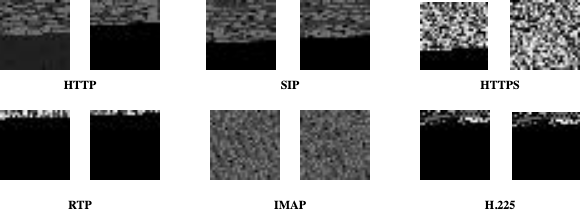
\includegraphics[width=\linewidth]{chapters/5/img/grayscaleimages.drawio.png}
\caption{Grayscale images generated from packets in our combined dataset used in the following experiments}
\label{fig:grayscale}
\end{figure}

To shape packet payloads into an image, we extract the payloads and convert them from byte encoding to a normalized decimal integer $i \in [0,255]$~\cite{jo2020packet}. For image size, we chose a $28\times28$ representation, for a total of 784 input features. Padding is applied in the cases where the payload is shorter than 784 bytes, and is otherwise truncated.

\subsection{LeNet Model Configuration}

\begin{figure} [ht!]
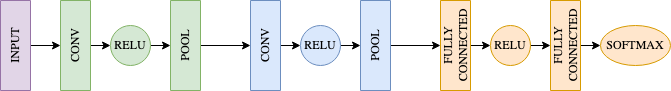
\includegraphics[width=\linewidth]{chapters/5/img/lenet.drawio.png}
\caption{The architecture of our LeNet models}
\label{fig:lenet}
\end{figure}

LeNet was one of the standard models we selected in order to test convolutional neural networks against the RTP detection problem. LeNet has a low complexity, so has higher potential for practical use in real-time, line-rate packet inspection systems than deeper models which require more time. Figure~\ref{fig:lenet} shows the set up of the model which we use as a baseline. We designed two separate models where one employed $6$ and $16$ kernels per convolutional layer (A) and another that used a $16$ and $32$ kernels (B). Each model contained two fully-connected, dense layers of size $1024$ with a binary softmax classifier at the output layer.

\subsection{ResNet Model Configuration}

\begin{figure} [ht!]
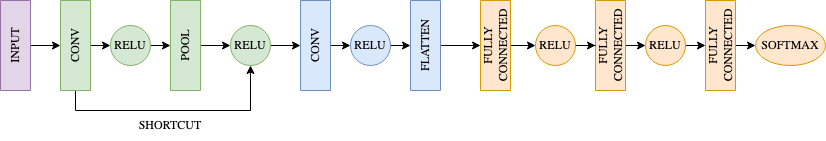
\includegraphics[width=\linewidth]{chapters/5/img/resnet.drawio.png}
\caption{The architecture of our ResNet models}
\label{fig:resnet}
\end{figure}

If they are to be deployed at scale, artificial intelligence solutions must be capable of line-rate processing while still being able to perform the classification task to the required level of accuracy. This can be difficult to quantify as the definition of line-rate varies per network environment. Still, we assert that the identity mappings of ResNet do not introduce additional complexity~\cite{resnet}. Thus, residual mapping is introduced as a potential solution to adding additional layers of representation and thus improve classification through more hidden features, while also minimizing overhead.

We developed four ResNet-based models for the \textsc{Maple} system's experiments. The first model (C) consists of three convolutional layers with $32$, $32$, and $64$ kernels of dimension $3\times3$, and three dense layers with output sizes of $64$, $32$, and $2$ respectively. The second model (D) follows a similar architecture except the values are halved. Convolutional layers had $16$, $16$, and $32$ kernels per layer and the three dense layers had output sizes of $32$, $16$, and $2$. Model (E) corresponds to the same number of kernels and output sizes as (C), except it uses a kernel dimension of $7\times7$. The ReLU activation function and adam optimizer was used in all the model configurations, and a final layer used softmax for normalization and classification. The loss function used for training was categorical cross-entropy, and we also employed a dropout layer to reduce overfitting.

\begin{table} [h!]
\centering
\begin{tabular}{| l | l | l | l | l |}
\hline
Type & Model & \# Kernels & Kernel Size & FC Dim \\
\hline
LeNet & A & $3\times3$ & 6, 16 & 1024, 2 \\
\cline{2-5}
& B & $3\times3$ & 16, 32 & 1024, 2 \\
\hline
ResNet & C & $3\times3$ & 32, 32, 64 & 64, 32, 2 \\
\cline{2-5}
& D & $3\times3$ & 16, 16, 32 & 32, 16, 2 \\
\cline{2-5}
& E & $7\times7$ & 32, 32, 64 & 64, 32, 2 \\
\cline{2-5}
\hline
\end{tabular}
\caption{Configurations of each model used in the experiments}
\label{table:attacks}
\end{table}
